\chapter{Synthetic geophysical experiments}
\label{SGE}
This chapter will outline a series of experiments which will test the main postulate of this thesis, that ABC can offer some improvement over traditional likelihood based Bayesian inference for geophysics. There are many potential avenues to pursue 'improvement'. For example, ABC opens parameter inference to models where there is no closed form expression for the likelihood. This can be used to compare the solution of parameter inference for a stochastic forward model where the data and modelization uncertainty do not conform to a Gaussian, to the solution obtained with the simplifying assumption that the uncertainty is Gaussian. This may constitute an improvement if it is shown that the ABC solution is significantly different from the analytical Gaussian solution. Here, instead of accurately assessing and utilizing the uncertainty in geophysical problems, other advantageous aspects of ABC are explored. Diagnostic parameter inference, which makes use of the information about the model contained in the simulated data, has been developed and applied \citep{Ratmann2009,vrugt2013toward}. Here diagnostic parameter inference for geophysics is explored with the goal of improving the rate an inversion algorithm moves toward a low misfit model. The benchmark for this test will be a MCMC algorithm targeting an analytically defined posterior. Currently there are many geophysical parameter inference problems where a probabilistic approach is required due to a trade-off between parameters, a non-unique parameter space or the availability of prior information. One example is an inversion for the thermal-chemical state of the lithosphere based on multiple different sets of constraining data \citep{afonso2013a,afonso2013b}. Currently exploring this 3D structure in high resolution is limited as the problem must be kept within the computational limits of the posterior sampling algorithm. If high resolution, many unknown parameters, and large scale, such as whole mantle 3D inversions, are to be implemented on problems which require a probabilistic formulation then methods which can efficiently find and define the set of low misfit models are required. Here a diagnostic ABC inversion may be able to improve the search for high probability (low misfit) models by taking into account more of the information available within the simulated dataset. \par

As with the previous chapter, the code to produce all figures in this section can be found at \url{https://github.com/tomconnell/approximate-bayesian-tomography}.\par


\section{Crustal density inversion}

As a first experiment, I consider an inversion for crustal density ($\rho$) with a vertical gravity anomaly dataset ($\Delta$ g) for a 2D discretized subsurface \citep[p.184-195,378]{blakely1996}. The dimensionality of the parameter space is kept modest, a 8x4 grid, with an observed data point above each column. The grid is defined over a 160 $km$ by 40 $km$ area. Density is bounded between 2-3.5 $g/cm^3$, the limits for which \citet{Brocher2005} define an empirical relationship between density and compressional-wave velocity ($V_p$). The 'true model', Figure \ref{true_model}, which will be the target of our inversion scheme, is kept smooth to allow a prior term, $p(\bm{\theta})$, to be set for smoothness which will limit the inversion to a unique solution. The definition for smoothness is:
\begin{equation}
-\text{log}\big(p(\bm{\theta})\big) = \sum_{i = 1}^{N} \Big(\sum_{j} (\rho_i - \rho_j)^2\Big)
\label{smoothness}
\end{equation}
where $j$ describes all blocks in immediate contact with the given block, $i$. The edge effect for the 2D subsurface grid is compensated by adding the vertical gravity anomaly which will result from extending the grid by a width of one on both sides, tripling the total domain width, with a density which is the average of the parameter space, 2.75 $g/cm^3$. The model is assumed to contain no modelization uncertainty and the data is known to be contaminated with noise defined by $\sigma^{\mathcal{D}} = \mathcal{N}(0,\sqrt{2})$.
\begin{figure}[H]
	\centering
	\includegraphics[scale=0.8]{true_model.pdf}
	\caption{The 'observed data', vertical component of gravity ($\Delta g$), and 'true model', a 2D density ($g/cm^3$) slice, which will be the target of our synthetic geophysical experiments to compare ABC to likelihood based Bayesian inference. A smoothness value, -log($p(\bm{\theta})$), equation \ref{smoothness}, for the true model is plotted for reference to later solutions.}
	\label{true_model}
\end{figure}
The benchmark for ABC-tomography to meet will be MCMC sampling of an analytically defined posterior. Given there is no modelization uncertainty and $\sigma^{\mathcal{D}}$ is known, the negative log-likelihood can be defined by, equation \ref{likelihood-1}:
\begin{equation}
	-l(\bm{\theta^*}|\bm{y}) = \frac{\sum_{i = 1}^{M}(y_i-y^*_i)^2}{(\sigma^{\mathcal{D}})^2}
	\label{analytical-applied-likelihood}
\end{equation}
For this section only MCMC is considered, no AM, DR or DRAM. This maintains a consistent sampling benchmark for comparison to the ABC scheme. The proposal distribution for both MCMC sampling of the analytical distribution and ABC-MCMC is held constant for all runs as $q(\cdot,\cdot) = \mathcal{N}(0,I\cdot250)$. The parameter space is subdivided into eight 2x2 blocks. At each time step a random block is selected in the subsurface and updated via $q(\cdot,\cdot)$. As demonstrated in table \ref{sampling-method-comparison}, the number of parameters updated at each time step impacts the acceptance rate and the rate of space exploration of the chain. To keep inference comparable both the analytical scheme and ABC scheme will update 4 parameters per time step via the proposal distribution. Likewise, for each experiment considered in this section the Markov chain starting position is the same for both the analytical MCMC and ABC-MCMC. The starting position for both is set by sampling a uniform distribution, $\mathcal{U}(2,3.5)$, to define each unknown parameter. \par

A set of summary statistics to describe the data in Figure \ref{true_model} is needed to proceed with ABC. A comprehensive description of the data is defined by the coefficients to a linear model, $m$ and $b$, the sample mean, $\bar{\mu_{\Delta g}}$, sample standard deviation, $\bar{\sigma_{\Delta g}}$, and a failsafe residual term, $\sum R$, for the difference between a simulation and the observed data for a given $\bm{\theta^*}$, $R = |\bm{y}-\bm{y^*}|$. Initial testing showed the set of statistics $\begin{bmatrix}
\bar{\mu_{\Delta g}}\ \bar{\sigma_{\Delta g}}\ m\ b\ \sum R
\end{bmatrix}^T$ comprehensively describes $\bm{y}$. As with section \ref{banana-section}, it is necessary to normalize the spread of each marginal distance term, $\text{d}_i(S_i(\bm{y}),S_i(\bm{y^*}))$, equation \ref{marginal_distance}, to one. This accounts for the different scales and sensitivities of the summary statistics to the unknown parameters. The normalization term $\bm{\sigma_S}$ is approximated from >10,000 Monte Carlo simulations over parameter range 2-3.5 $g/cm^3$. The tolerance is closely related to the acceptance rate of the algorithm. Given the tolerance is tightly tied to the acceptance rate, the tolerance is tuned to balance accuracy and acceptance rate.\par

\citet{Sisson2010a} highlight that sampler acceptance rate and mixing can be improved by increasing the number of simulated datasets, $\bm{y^*}$, for each set of model parameters, $\bm{\theta^*}$. This is a technique also adopted in applications with large uncertainty in $\bm{g_s}$ \citep{Ratmann2009,Wood2010}. This has a stabilizing impact when the uncertainty in each simulation is large. The set of simulated data make up a Monte Carlo approximation to the true value of the ABC likelihood ($p(\bm{y}|\bm{y^*},\bm{\theta})$) which would be found as the number of simulated datasets tends to $\infty$. Hence, the estimate of the ABC likelihood for a given set of parameters becomes less noisy as the number of simulated datasets increases. This technique is used for $k = 100$ simulations from $\bm{g_s}$. Since the bulk of the computational overhead is in solving the deterministic physical model and the data uncertainty is additive and fast to simulate, there is little computational cost in increasing  the number of simulated datasets. The distance is then computed based the sample mean of $\bm{y^*_{1:k}}$, $\bm{d} = |\bm{S}(\bm{y})-\bm{S}(\bm{\bar{\mu_{y^*}}})|$. \par

The diagnostic ABC scheme is free to open the likelihood, consider the information available, and use that to make an informed next step in the Markov chain. The ABC scheme moves away from randomly selecting 2x2 blocks in the subsurface to update as is done in the analytical MCMC scheme. Instead, the update is selected to ensure that it is occurring in a location where the current fit of the simulated data to the observed data is poor. A discrete PDF is defined over each data point which is proportional to the misfit:
\begin{equation}
	p(\text{update}) \propto \text{misfit} = (\bm{y}-\bm{y^*})^2
	\label{misfit}
\end{equation}
A random sample from this PDF is then drawn at each time step to determine where the parameter updates will occur. Once a data point is selected the 4 parameters directly below are updated. The effectiveness of dynamically selecting and localizing the updates relies on our physical intuition about the relationship between the unknown model parameters and the resulting data. In this case, each simulated data point is most sensitive to the parameters which are directly below it, and by focusing model updates on regions which are poorly fitting, the most is made from each move during the initial phase of the algorithm where rapid local transitions are made in search of an area of high posterior density. This change has ideas similar to the way gradient-based linear optimization methods work, however, here I simply rely on physical intuition within a Bayesian framework. \par

As a next step in defining a diagnostic ABC inversion, the proposal distribution is directed to bias the parameter updates in the direction which the simulated data needs to move to lower the misfit. For example, if a data point is selected based on sampling the discrete PDF equation \ref{misfit} and it is found the simulate data point is too large, i.e. the value $y^*_{\Delta g} - y_{\Delta g}$ is positive, then the proposal for the column of parameters at this update step will be biased towards a density lower than the current parameter value. In this case a truncated Gaussian distribution , figure \ref{updates}, is used to bias the proposal updates. For the example where the currently selected data point is too large, the update can be biased toward a lower density by sampling a truncated Gaussian distribution, centered at the current chain location, and truncated at some position greater than the current chain location. A truncated Gaussian is convenient to implement as detailed balance is satisfied without computing the ratio $\frac{q(\bm{\theta^*},\bm{\theta_{t-1}})}{q(\bm{\theta_{t-1}},\bm{\theta^*})}$ at each time step. \par

The analytical definition for the truncated normal distribution, $f(x)$, used to direct the parameter updates is:
\begin{equation}
f(x) = \begin{cases} 
0 & x < a \\
\frac{1}{\sqrt{2\pi\sigma^2}}\text{exp}\Big(-\frac{(x-\mu)^2}{2\sigma^2}\Big) & a\leq x\leq b \\
0 & x > b 
\end{cases}
\label{trunc-eq}
\end{equation}
Here $a$ is the lower cut-off and $b$ is the upper cut-off. In this application the negatively truncated distribution has $a = -\frac{1}{2}\sigma$ and $b = \infty$. While the positively truncated distribution has $a = -\infty$ and $b = \frac{1}{2}\sigma$. For our application $\mu$ is the current chain location and $\sigma$ = 250. \par

\begin{figure}[H]
	\centering
	\includegraphics[scale=1.1]{updates.pdf}
	\caption{The proposal distributions which are used to either positively or negatively bias the parameter update. The negatively truncated Gaussian distribution (a) is used when the parameter values are deemed too low. The positively truncated Gaussian distribution (b) is used when the parameter values are deemed too high. Equation \ref{trunc-eq} defines the truncated Gaussian distribution. During application the distributions are centered on the current chain location and $\sigma = 250$. The cut-off $a$ and $b$ are selected to set the bias at 70\% to 30\%.} 
	\label{updates}
\end{figure}


Figure \ref{comparison-1} plots a comparison between the misfit, equation \ref{misfit}, for the analytical scheme described above and diagnostic ABC scheme during the initial phase (first 10,000 time steps) of their respective Markov chains. The dynamically selection and directing of parameter updates increases the rate at which the ABC algorithm moves to a low misfit model significantly in comparison to a traditional analytical MCMC scheme. Figure \ref{ana-im-1} and \ref{abc-im-1} plot the solution obtained, mean marginal model, for the full chain (100,000 time steps).\par

\begin{figure}[H]
	\centering
	\includegraphics[scale=0.7]{comparison.pdf}
	\caption{The misfit, l2-norm, equation \ref{misfit}, for the chain state during the optimization phase (first 10,000 time steps) for an analytically defined posterior compared to ABC-tomography. The 'true model' and observed data is plotted in figure \ref{true_model}. Both posteriors, analytical and ABC-tomography, use a parameter space bound between 2-3.5 $g/cm^3$ and a prior 'smoothness' defined by equation \ref{smoothness}. The speed increase in optimization is a result of opening the likelihood and using the information contained in each iteration to localize the next update to an area where the current data fit is poor. The details of the full chain run, 100,000 time steps, are also displayed on the figure. $\tau$ is the integrated auto-correlation time.}
	\label{comparison-1}
\end{figure}

\begin{figure}[H]
	\centering
	\includegraphics[scale=0.8]{ana_im.pdf}
	\caption{The mean of the marginal posterior, $p(\bm{\theta}|\bm{y})$, defined by the prior equation \ref{smoothness} and likelihood \ref{analytical-applied-likelihood} targeting the 'true model' and observed data of figure \ref{true_model}. The simulated data generated by this 'solution' is plotted, red, compared to the observed data, black. The smoothness, equation \ref{smoothness}, and misfit, equation \ref{misfit}, for this model are displayed alongside the data. The misfit during the optimization phase for this chain is plotted in figure \ref{comparison-1}. This model can be compared to the equivalent for the ABC-tomography chain, figure \ref{abc-im-1}.}
	\label{ana-im-1}
\end{figure}

\begin{figure}[H]
	\centering
	\includegraphics[scale=0.8]{abc_im.pdf}
	\caption{The mean of the marginal ABC posterior, $p_{ABC}(\bm{\theta}|\bm{S}(\bm{y}))$, targeting the 'true model' and observed data of figure \ref{true_model}. The simulated data generated by this 'solution' is plotted, blue, compared to the observed data, black. The smoothness, equation \ref{smoothness}, and misfit, equation \ref{misfit}, for this model are displayed alongside the data. The misfit during the optimization phase for this chain is plotted in figure \ref{comparison-1}. This model can be compared to the equivalent for the analytically defined posterior, figure \ref{ana-im-1}.}
	\label{abc-im-1}
\end{figure}



\section{Crustal density joint inversion}

As a second experiment I extend the inversion for crustal density ($\rho$) for a 2D discretized subsurface to a joint inversion with vertical gravity anomaly ($\Delta$ g) and travel times for compressional-waves $V_p$. Both datasets share the same underlying parameter space in $\rho$. The calculation for $V_p$ is made through the empirical relationship for $V_p$ as a function of $\rho$ defined by \citet{Brocher2005}:
\begin{equation}
	V_p\ (km/sec) = 0.8228\rho^5 - 9.1819\rho^4 + 37.0.83\rho^3 - 63.064\rho^2 + 39.128\rho
	\label{rhotovp}
\end{equation}
This relationship is valid for crustal rocks with $\rho$ in the range of 2-3.5 $g/cm^3$. As with the first example the 'true model' is kept smooth and the prior equation \ref{smoothness} is used. The parameter space is expanded to a 20x6 grid over the same 160 $km$ by 40 $km$ area. There is a $\Delta$g measurement made above each of the 20 columns. Both the $\Delta$g and $\Delta t$ (travel-time based on $V_p$) dataset are contaminated with measurement uncertainty defined by $\sigma^{\mathcal{D}} = \mathcal{N}(0,\sqrt{2})$. As before, the benchmark for ABC-tomography will be MCMC sampling of an analytically defined posterior. The likelihood for this problem is based on \ref{joint-likelihood}, with a negative log-likelihood defined as:
\begin{equation}
	-l(\bm{\theta}|\bm{y}) = \frac{c(\bm{y_{\Delta g}}-\bm{y^*_{\Delta g}})^2}{(\sigma^{\mathcal{D}})^2} + \frac{(\bm{y_{V_p}}-\bm{y^*_{V_p}})^2}{(\sigma^{\mathcal{D}})^2}
\end{equation}
where $c$ is a constant defined so as the contribution to the negative log-likelihood of both datasets is of the same order of magnitude. The proposal distribution is held as $q(\cdot,\cdot) = N(0,I\cdot250)$ however, given the increased parameter space the subsurface is divided into 20 2x3 blocks. A random block is selected for update at each time step in the analytical scheme. The starting position is initialized from $\mathcal{U}(2,3.5)$  and once again held constant between both the analytical Markov chain and ABC-tomography. \par

I once again seek a comprehensive set of summary statistics to describe $\bm{y_{\Delta g}}$ and $\bm{y_{V_p}}$. The set $\begin{bmatrix}
\bar{\mu_{\Delta g}}\ \bar{\sigma_{\Delta g}}\ m\ b\ \sum R
\end{bmatrix}^T$ is used for $\bm{y_{\Delta g}}$. Given $\bm{y_{V_p}}$ is the vector for arrival times for each source. Instead of fitting statistics to the larger $\bm{y_{V_p}}$, $\bm{y_{V_p}}$ is decomposed to the set of data for each source, 1 to $l$, where $l$ is the number of sources. The arrivals from each individual source are then described by $\begin{bmatrix}
m\ b\ \sum R
\end{bmatrix}^T$. The weighting kernel for $\bm{y_{V_p}}$ then becomes:
\begin{equation}
	p(\bm{y_{V_p}}|\bm{y^*_{V_p}},\bm{\theta^*}) = \prod_{i = 1}^{l} p(\bm{y_i}|\bm{y^*_i},\bm{\theta^*})
\end{equation}
A normalization term $\bm{\sigma_S}$ is approximated for both datasets from >10,000 Monte Carlo simulations over parameter range 2-3.5 $g/cm^3$. \par

For ABC-tomography I again open the likelihood at each time step and consider the information available to localize the parameter updates. The 6 parameters below a given data point are updated based on Monte Carlo sampling of a probability distribution proportional to the misfit of the $\bm{y_{\Delta g}}$ data set. For this joint inversion I extend the ABC-tomography scheme based on physical intuition by both dynamically selecting and localizing the update, and directing the proposal to bias the update in the direction which the data needs to go. This is done through the use of a skew Gaussian distribution or alternatively a truncated Gaussian distribution. These distributions are then adjusted to bias the update in either a positive or negative direction. If, for example, a gravity anomaly is selected by sampling the misfit distribution and it is found to be too large, i.e the value $y^*_{\Delta g} - y_{\Delta g}$ is positive, then the proposal for the column of parameters at this update step can either be sampled from: a negatively skewed Gaussian distribution centered on the current chain position; or a truncated Gaussian distribution, which is truncated at some position greater than the current chain position. \par
It should be noted that when using the skew normal distribution, as it is not a symmetric distribution, the ratio $\frac{q(\bm{\theta^*},\bm{\theta_{t-1}})}{q(\bm{\theta_{t-1}},\bm{\theta^*})}$ must be computed at each time step to ensure detailed balance is maintained. \par

\begin{figure}[H]
	\centering
	\includegraphics[scale=0.75]{true_model_gravity.pdf}
	\caption{The 'observed data', vertical component of gravity ($\Delta g$), and 'true model', a 2D density ($g/cm^3$) slice, which will be the target of our synthetic geophysical experiments to compare ABC to likelihood based Bayesian inference. A smoothness value, log($p(\bm{\theta})$), equation \ref{smoothness}, for the true model is plotted for reference to later solutions.}
	\label{true-model-large-grav}
\end{figure}

\begin{figure}[H]
	\centering
	\includegraphics[scale=0.75]{observed_tomography.pdf}
	\caption{The 'true model', a 2D $Vp$ ($km/s$) slice, converted from $\rho$ by the empirical relationship defined by equation \ref{rhotovp}. The black lines across the model define the rays from 12 sources on their path to 10 receivers. The arrival time $\Delta t$ of these rays at the receivers defines the 'observed data'. A sample of observed data is plotted for 4 sources. The sources are numbered 1-12 starting from the top left and going to the top right, with 4 sources per side.}
	\label{true-model-tom}
\end{figure}


The analytical definition for the skew normal distribution, $f(x)$, used to direct the parameter updates is:
\begin{equation}
\begin{split}
\phi(x) = \frac{1}{\sqrt{2\pi}}\text{exp}\Big(-\frac{x^2}{2}\Big) \\
\Phi(x) = \frac{1}{2}\bigg(1 + \text{erf}\Big(\frac{x}{\sqrt{2}}\Big)\bigg)\\
f(x) = \frac{2}{\omega} \phi\bigg(\frac{x-\xi}{\omega}\bigg)\Phi\bigg(\alpha \Big(\frac{x-\xi}{\omega}\Big)\bigg)
\end{split}
\label{skew-normal-dist}
\end{equation}
here erf is the error function, $\xi$ is the location, $\omega$ is the scale and $\alpha$ is a shape parameter. In this application  $\xi$ is the current chain location, $\omega$ is held at 250, and $\alpha$ is either 1, for a positively skewed distribution, or -1, for a negatively skewed distribution. \par
The analytical definition for the truncated normal distribution, $f(x)$, used to direct the parameter updates is:
\begin{equation}
	f(x) = \begin{cases} 
	0 & x < a \\
	\frac{1}{\sqrt{2\pi\sigma^2}}\text{exp}\Big(-\frac{(x-\mu)^2}{2\sigma^2}\Big) & a\leq x\leq b \\
	0 & x > b 
	\end{cases}
	\label{trunc-eq}
\end{equation}
Here $a$ is the lower cut-off and $b$ is the upper cut-off. In this application the negatively truncated distribution has $a = -\frac{1}{2}\sigma$ and $b = \infty$. While the positively truncated distribution has $a = -\infty$ and $b = \frac{1}{2}\sigma$. For our application $\mu$ is the current chain location and $\sigma$ = 250. \par
Figure \ref{updates} plots the directed proposal distributions described above and applied in ABC-tomography. Figure \ref{updates}(a)(b) are used when the parameter values need to be lowered, and figure \ref{updates}(c)(d) are used when the parameter values need to be increased. 

\begin{figure}[H]
	\centering
	\includegraphics[scale=1]{updates.pdf}
	\caption{The proposal distributions which are used to either positively or negatively bias the parameter update. The negatively skewed Gaussian distribution in (a) and the positively truncated Gaussian distribution in (b) are used to bias the proposal when the parameter values are deemed too high. The positively skewed Gaussian distribution (c) and the negatively truncated Gaussian distribution zre used when the parameter values are deemed too low. Equation \ref{skew-normal-dist} defines the skew Gaussian distribution while equation \ref{trunc-eq} defines the truncated Gaussian distribution. During application the distributions are centered on the current chain position, and $\sigma = \omega = 250$. The shape parameter, $\alpha$, and cut-off, $a$ and $b$ are selected to set the bias at approximately 70\% to 30\%.}
	\label{updates}
\end{figure}

Figure \ref{comparison-trunc} and \ref{comparison-skew} plots a comparison between the normalized misfit for the analytical scheme and ABC-tomography during the optimization phase of their respective Markov chains for both skew Gaussian and truncated Gaussian updates. This shows how the speed of optimization can be improved through opening the likelihood and allowing the simulated data to select, localize and direct the parameter updates. While it should be noted that the acceptance rate collapses when compared to undirected ABC-tomography, each move is more informed and the quality of next move in the chain is higher (i.e the misfit is lower). Figure \ref{grav-trunc}, \ref{tom-trunc}, \ref{grav-skew}, and \ref{tom-skew} plot the mean marginal model for the full chain lengths. This demonstrates the accuracy of the recovered solutions. \par

\begin{figure}
	\centering
	\includegraphics[scale=0.8]{comparison-trunc.pdf}
	\caption{Truncated Gaussian scheme. The normalized misfit of the chain state during the optimization phase (first 10,000 steps) for both datasets, $\Delta g$ and $\Delta t$, and for both methods, an analytically defined posterior sampled by MCMC and ABC-tomography. The 'true model' and observed data is plotted in figure \ref{true-model-large-grav} and \ref{true-model-tom}. The increase in optimization time under ABC-tomography is a result of dynamically selecting, localizing and directly the update at each time step in the Markov chain. The details of the full chain run (100,000 time steps), are also displayed on the figure. $\tau$ is the integrated auto-correlation time. The mean marginal models from ABC-tomography using truncated Gaussian updates is plotted in figure \ref{grav-trunc} and \ref{tom-trunc}.}
	\label{comparison-trunc}
\end{figure}

\begin{figure}
	\centering
	\includegraphics[scale=0.7]{abc_im-trunc.pdf}
	\caption{Truncated Gaussian scheme. The mean of the marginal ABC posterior, $p_{ABC}(\bm{\theta}|\bm{S}(\bm{y}))$, targeting the 'true model' and observed data of figure \ref{true-model-large-grav}. The simulated data generated by this 'solution', is plotted, blue, compared to the observed data, black. The misfit during the optimization phase for this chain is plotted in figure \ref{comparison-trunc}. The corresponding mean marginal $V_p$ model is plotted in figure \ref{tom-trunc}.}
	\label{grav-trunc}
\end{figure}

\begin{figure}
	\centering
	\includegraphics[scale=0.7]{abc-trunc}
	\caption{Truncated Gaussian scheme. The mean of the marginal ABC posterior, $p_{ABC}(\bm{\theta}|\bm{S}(\bm{y}))$, targeting the 'true model' and observed data of figure \ref{true-model-tom}. The simulated data generated by this 'solution', is plotted, blue, compared to the observed data, black. The misfit during the optimization phase for this chain is plotted in figure \ref{comparison-trunc}. The corresponding mean marginal $\rho$ model is plotted in figure \ref{grav-trunc}.}
	\label{tom-trunc}
\end{figure}

\begin{figure}
	\centering
	\includegraphics[scale=0.6]{comparison-skew.pdf}
	\caption{Skew Gaussian scheme. The normalized misfit of the chain state during the optimization phase (first 10,000 steps) for both datasets, $\Delta g$ and $\Delta t$, and for both methods, an analytically defined posterior sampled by MCMC and ABC-tomography. The 'true model' and observed data is plotted in figure \ref{true-model-large-grav} and \ref{true-model-tom}. The increase in optimization time under ABC-tomography is a result of dynamically selecting, localizing and directly the update at each time step in the Markov chain. The details of the full chain run (100,000 time steps), are also displayed on the figure. $\tau$ is the integrated auto-correlation time. The mean marginal models from ABC-tomography using skew Gaussian updates is plotted in figure \ref{grav-skew} and \ref{tom-skew}.}
	\label{comparison-skew}
\end{figure}

\begin{figure}
	\centering
	\includegraphics[scale=0.7]{abc_im-skew.pdf}
	\caption{Skew Gaussian scheme. The mean of the marginal ABC posterior, $p_{ABC}(\bm{\theta}|\bm{S}(\bm{y}))$, targeting the 'true model' and observed data of figure \ref{true-model-large-grav}. The simulated data generated by this 'solution', is plotted, blue, compared to the observed data, black. The misfit during the optimization phase for this chain is plotted in figure \ref{comparison-skew}. The corresponding mean marginal $V_p$ model is plotted in figure \ref{tom-skew}.}
	\label{grav-skew}
\end{figure}

\begin{figure}
	\centering
	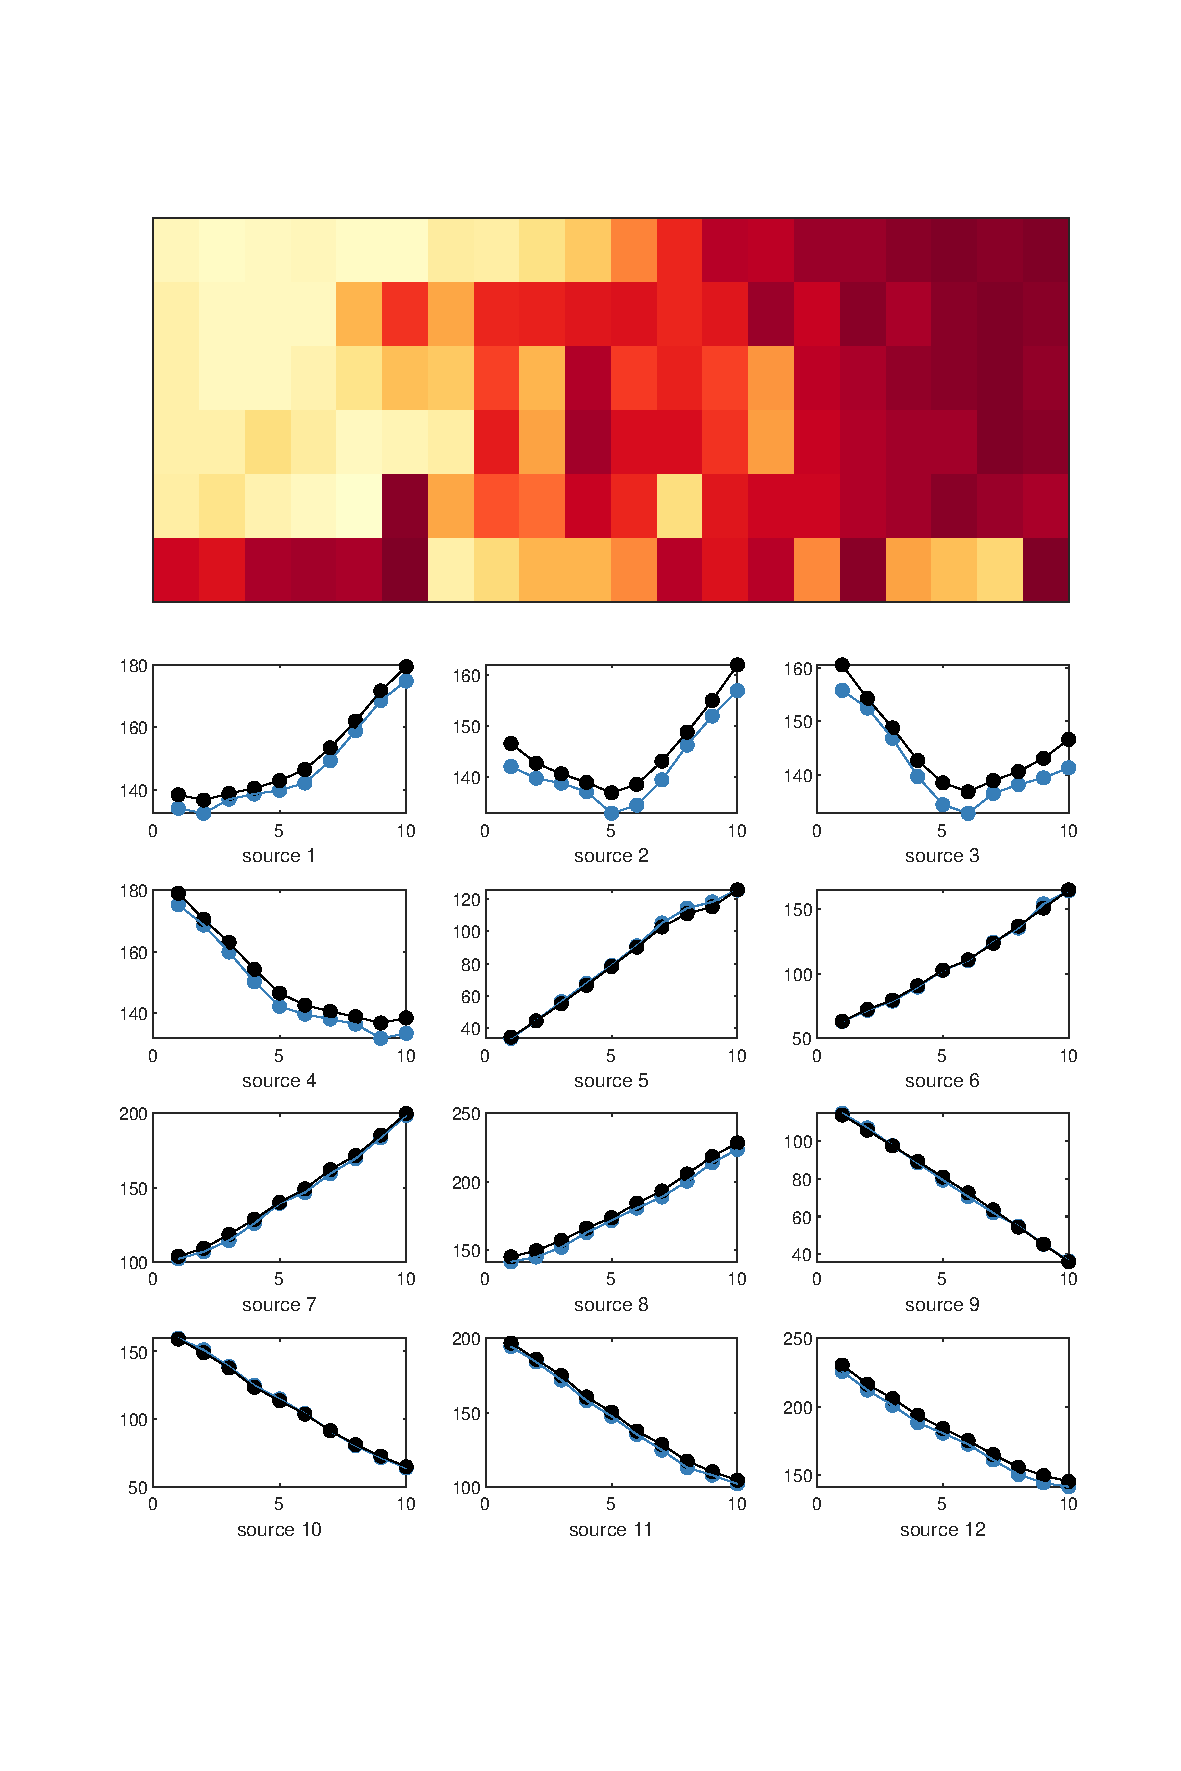
\includegraphics[scale=0.7]{abc-skew.pdf}
		\caption{Skew Gaussian scheme. The mean of the marginal ABC posterior, $p_{ABC}(\bm{\theta}|\bm{S}(\bm{y}))$, targeting the 'true model' and observed data of figure \ref{true-model-tom}. The simulated data generated by this 'solution', is plotted, blue, compared to the observed data, black. The misfit during the optimization phase for this chain is plotted in figure \ref{comparison-skew}. The corresponding mean marginal $\rho$ model is plotted in figure \ref{grav-skew}.}
	\label{tom-skew}
\end{figure}


